\section{Topic Tree}

The topic tree feature will be examined based on a framework to determine how well the implemented feature has achieved its intended purpose and its functionality. \\

Therefore the analysis includes four sections:\\
\begin{enumerate}
    \item Functional Requirements - does the system fulfil the functional requirements set out in the project approach?
    \item Non-functional requirements - how well does the system achieve the non functional requirements including performance and accessibility
    \item Scalability and Efficiency - how well does the feature perform with many, many topics and topic groups?
    \item Feedback from potential users of the feature - what do users such as lecturers, tutors and students think about the feature and how could it be improved?
\end{enumerate}

\subsection{Functional requirements}
The functional requirements of the feature were analysed for completedness. Each functional requirement has a priority attached to it, and the functionality of the system was assessed against this priority. \\

In total, 15 requirements out of 18 were fully completed. 1 high requirement, 1 medium requirement and 1 low requirement were not completed at all. 9 high requirements, 5 medium requirements and 1 low requirement were completed. \\

The following explains the requirements that were not completed and why they were not completed.\\
\\
\textbf{Users can search for specific resources - High Priority} \\
Currently the topic tree feature allows users to search through the topic tree for specific topics, but does not allow users to search through the entire topic tree for a specific resource. This is because topic resources are already grouped by topic, and there was no need to have to search the entire topic tree for a specific resource. Also, tags were added as a feature where users can specify different synonyms for a topic, improving searchability. Topic resources is also commonly given generic names, such as "Lecture Slides". This is not descriptive of the content, and would have proved resource searchability difficult. \\
\\
\textbf{Users can delete a topic group that they've created - Medium Priority}\\
Users can currently create topic groups, but cannot delete them. This is due to integration issues found with deleting topics, as topic groups are an integral part of the entire system. Deleting topic groups could create database integrity issues, and there was not enough time to fix these issues.\\
\\
\textbf{Users can export data from topics and course material - Low Priority} \\
This requirement was classed low priority as the system was designed to be the only learning management system for an entire faculty or university. Exporting data from topics and course material would have proved useful for exporting into another learning management system, but there was again not enough time to implement this feature either.\\

\subsection {Non functional requirements}

The following details the analysis undertaken to examine the accessibility, security and performance of the feature. 

\subsection {Performance}

Performance of the system could be improved, with the main topic tree graph view loading a little slowly. Google Lighthouse was used to analyse performance, and performance differs depending on the database server used i.e. if a remote server was used, the topic tree takes longer to load the graph.\\

Google Lighthouse is a tool used to measure page performance and accessibility, and gives a score out of 100 after running its tests. It waits until there is no more movement on the graph and measures the time taken, however the page is interactive before movement stops on the graph due to nodes slowly moving outwards from where they loaded.\\


\begin{figure}[h!]
    \centering
    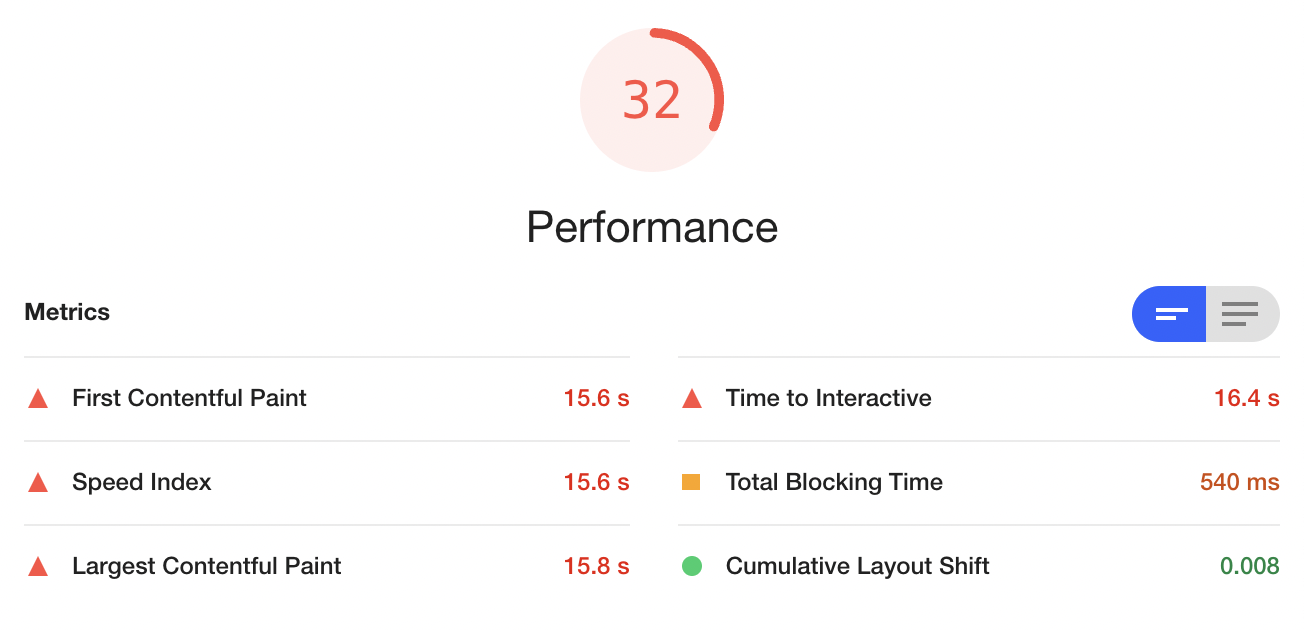
\includegraphics[scale=0.4]{topic-tree-performance}
    \caption{Performance report of the topic tree}
\end{figure}

As shown in the report, a score of 32/100 was given for the topic tree's performance. Restructuring of the database and less API requests are strategies that can be used to improve the performance of the topic tree, as well as a different graphing library as d3 is not an optimised library for handling graphs.\\

\subsection{Accessibility}
Accessibility of the feature is good, as the Chakra UI library was used to ensure that alt and aria tags were used. Colour contrast of the feature could be improved, but is still quite good with contrasting blue and white colours used. \\

\begin{figure}[h!]
    \centering
    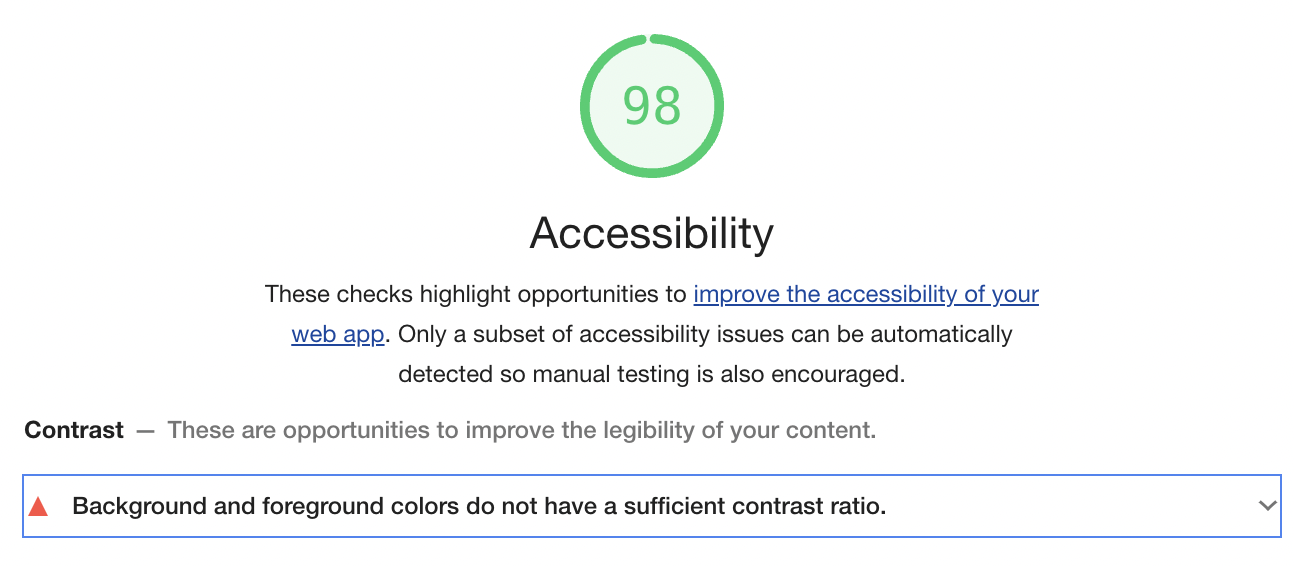
\includegraphics[scale=0.4]{topic-tree-accessibility}
    \caption{Accessibility report of the topic tree}
\end{figure}

A score of 98 was achieved for accessibility. Google Lighthouse accesses tags and HTML elements used, as well as contrast ratios to assess accessibility.\\

\subsection{}